\begin{blocksection}
\question What would Python display? Draw box-and-pointer diagrams for the following:

\begin{lstlisting}
>>> a = [1, 2, 3]
>>> a
\end{lstlisting}
\begin{solution}[.25in]
\begin{lstlisting}
[1, 2, 3]
\end{lstlisting}
\end{solution}

\begin{lstlisting}
>>> a[2]
\end{lstlisting}
\begin{solution}[.25in]
3
\end{solution}

\begin{lstlisting}
>>> a[-1]
\end{lstlisting}
\begin{solution}[.25in]
3
\end{solution}

\end{blocksection}
\begin{blocksection}

\begin{lstlisting}
>>> b = a
>>> a = a + [4, [5, 6]]
>>> a
\end{lstlisting}
\begin{solution}[.25in]
\begin{lstlisting}
[1, 2, 3, 4, [5, 6]]
\end{lstlisting}
\end{solution}
\begin{lstlisting}
>>> b
\end{lstlisting}
\begin{solution}[.25in]
\begin{lstlisting}
[1, 2, 3]
\end{lstlisting}
\end{solution}

\end{blocksection}
\begin{blocksection}

\begin{lstlisting}
>>> c = a
>>> a = [4, 5]
>>> a
\end{lstlisting}
\begin{solution}[.25in]
\begin{lstlisting}
[4, 5]
\end{lstlisting}
\end{solution}

\begin{lstlisting}
>>> c
\end{lstlisting}
\begin{solution}[.25in]
\begin{lstlisting}
[1, 2, 3, 4, [5, 6]]
\end{lstlisting}
\end{solution}
\end{blocksection}

\begin{blocksection}

\begin{lstlisting}
>>> d = c[3:5]
>>> c[3] = 9
>>> d

\end{lstlisting}
\begin{solution}[.25in]
\begin{lstlisting}
[4, [5, 6]]
\end{lstlisting}
\end{solution}

\begin{lstlisting}
>>> c[4][0] = 7
>>> d
\end{lstlisting}
\begin{solution}[.25in]
\begin{lstlisting}
[4, [7, 6]]
\end{lstlisting}
\end{solution}
\end{blocksection}
\begin{blocksection}
\begin{lstlisting}
>>> c[4] = 10
>>> d
\end{lstlisting}
\begin{solution}[.25in]
\begin{lstlisting}
[4, [7, 6]]
\end{lstlisting}
\end{solution}

\begin{lstlisting}
>>> c
\end{lstlisting}
\begin{solution}[.25in]
\begin{lstlisting}
[1, 2, 3, 9, 10]
\end{lstlisting}
\end{solution}

\end{blocksection}
    
\begin{solution}[0in]
\begin{blocksection}
\textbf{Shared Nested List}

Immediately after \lstinline{c[4][0] = 7}, the lists referenced by
\lstinline{c} and \lstinline{d} share the same inner list. Only these
two variables are shown.
\begin{center}
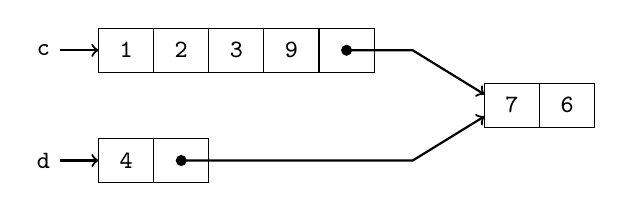
\begin{tikzpicture}[x=0.7cm,y=0.7cm, every node/.style={font=\small\ttfamily}]
    \node (cname) at (0,2) {c};
    \draw (1,1.6) rectangle (6,2.4);
    \foreach \x in {2,3,4,5} {\draw (\x,1.6) -- (\x,2.4);}
    \node at (1.5,2) {1};
    \node at (2.5,2) {2};
    \node at (3.5,2) {3};
    \node at (4.5,2) {9};
    \fill (5.5,2) circle (2pt);
    \draw[->,thick] (cname.east) -- (1,2);
    \node (dname) at (0,0) {d};
    \draw (1,-0.4) rectangle (3,0.4);
    \draw (2,-0.4) -- (2,0.4);
    \node at (1.5,0) {4};
    \fill (2.5,0) circle (2pt);
    \draw[->,thick] (dname.east) -- (1,0);
    \draw (8,0.6) rectangle (10,1.4);
    \draw (9,0.6) -- (9,1.4);
    \node at (8.5,1) {7};
    \node at (9.5,1) {6};
    \draw[->,thick] (5.5,2) -- (6.7,2) -- (8,1.2);
    \draw[->,thick] (2.5,0) -- (6.7,0) -- (8,0.8);
\end{tikzpicture}
\end{center}
The next assignment, \lstinline{c[4] = 10}, replaces the reference
in \lstinline{c}; \lstinline{d[1]} still points to \lstinline{[7, 6]}.

\href{https://pythontutor.com/visualize.html#code=a%20%3D%20%5B1,%202,%203%5D%0Aa%0Aa%5B2%5D%0Aa%5B-1%5D%0A%0Ab%20%3D%20a%0Aa%20%3D%20a%20%2B%20%5B4,%20%5B5,%206%5D%5D%0Aa%0Ab%0A%0Ac%20%3D%20a%0Aa%20%3D%20%5B4,%205%5D%0Aa%0Ac%0A%0Ad%20%3D%20c%5B3%3A5%5D%0Ac%5B3%5D%20%3D%209%0Ad%0A%0Ac%5B4%5D%5B0%5D%20%3D%207%0Ad%0A%0Ac%5B4%5D%20%3D%2010%0Ad%0Ac&mode=edit&origin=opt-frontend.js&py=311}{Click this text and share this link with students; this link renders Python Tutor diagram of this question.}
\end{blocksection}
\end{solution}

\begin{meta}
\noindent
\begin{blocksection}
\textbf{How to Draw Lists}

Draw one box per list element and label the indices starting at zero. Draw arrows from variable names to their list objects, and from list elements to any nested lists. When two arrows reach the same object, changing that object is visible through both references. In this question, contrast creating a new outer list with changing a shared nested list. Use the solution diagram and Python Tutor link after students have made their predictions.
\end{blocksection}\par
\end{meta}

\begin{questionmeta}
    \textbf{Teaching Tips}
    \begin{enumerate}
            \item Draw box-and-pointer diagrams on the board: use one box per list element and arrows for references to nested lists.
            \item Encourage students to draw box and pointer diagrams if they seem stuck
            \item It can be helpful to visually go through indexing and list slicing in the box and pointer diagram
            \item Python is confusing when adding on to a list with \lstinline{lst += [element]} and \lstinline{lst = lst + element}. The former mutates and the latter creates a new list
            \item Make sure you clearly state when you’re making a new list object (i.e. at \lstinline{a = a + [4, [5, 6]]} and list slicing like \lstinline{d = c[3:5]})
            \item Be sure to touch on negative indices and reiterate the difference between shallow and deep copies -- as it's a nuance in list comprehension, we decided not to include it in the overview, but when going over this problem, please make sure to touch on this!
            \item If students need additional help with shallow and deep copying, feel free to come up with your own creative iterations on the shallow and deep copying problems.
    \end{enumerate}
\end{questionmeta}

\begin{questionmeta}
    Suggested Time: 8--12 min; Difficulty: Easy--Medium
    Prioritize positive, negative, and nested indexing. Treat later mutation cases as an extension. Distinguish rebinding a name from changing a list; slices make a new outer list with references to the same elements.
\end{questionmeta}
